\chapter{Limits and Troubles}


\section{Communication Failure: Two Armies Problem}
\begin{figure}
\centering
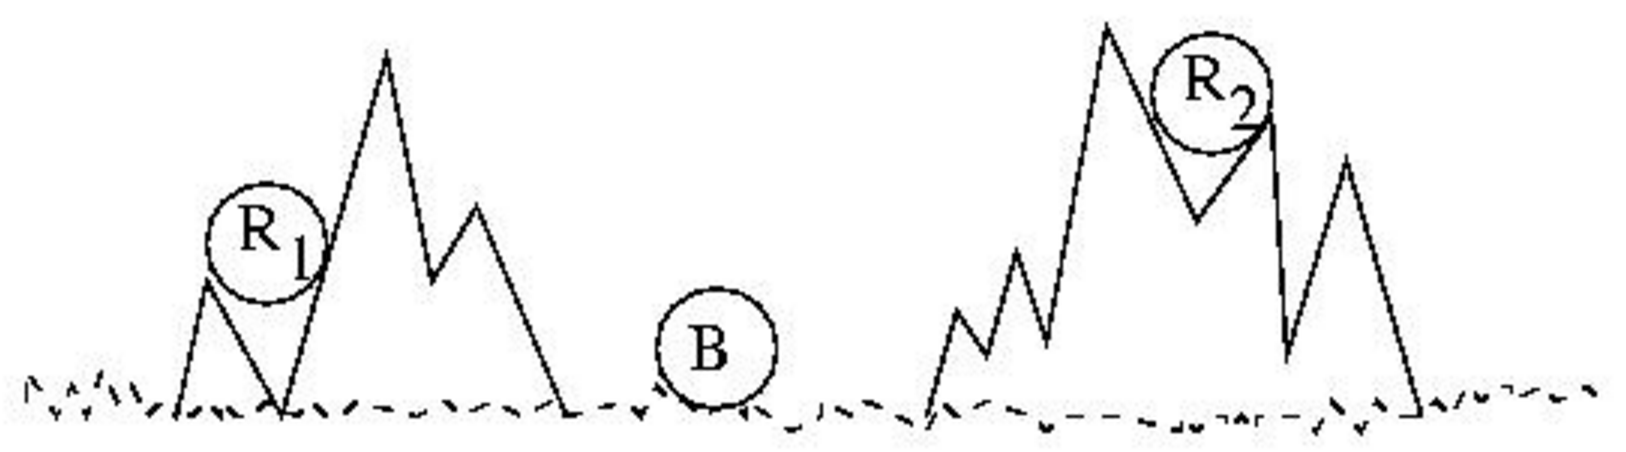
\includegraphics[width=\textwidth]{img/ch07-twoarmies.png}
\caption{Two Armies}
\label{fig:ch07-twoarmies}
\end{figure}

\begin{enumerate}
    \item Attack at the same time.
    \item Fake messages.
\end{enumerate}

The moral of this story is that there is no solution to this probem if the communications medium is unreliable. Please note that I said medium, not protocol.

\section{Processor Failure: Byzantine Problem}

\begin{enumerate}
    \item Traitor
\end{enumerate}

If the disloyal general tells the same lie to all of the generals, they will each agree to the wrong value. For this reason, based on this pedagogical story, undetectible errors (faulty hardware, not faulty communications) are known as Byzantine Errors by computer scientists.

The moral of this story is that failures can be expensive to detect -- sometimes impossible. This means that distributed agreement may not be expensive -- or impossible. Sometimes we have to pay the price, sometimes we don't. The successful design and implementation of distributed systems depending on knowing what we can do.

\section{CAP Conjecture}
\begin{itemize}
    \item Consistency
    \item Availability
    \item Partition Tolerance
\end{itemize}
The CAP Conjecture is that we can build systems that guarantee up to two of these properties -- but not necessarily all three. 

\subsubsection{}
\begin{figure}
\centering
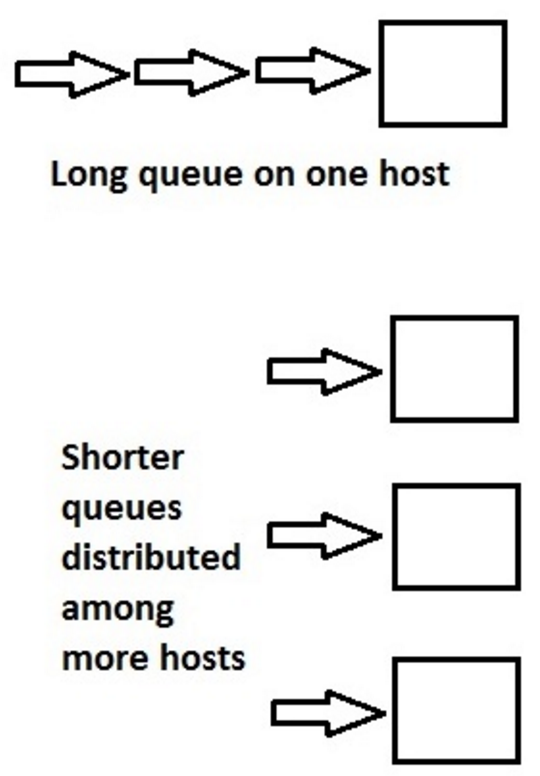
\includegraphics[width=0.5\textwidth]{img/ch07-apcase.png}
\caption{AP Case}
\label{fig:ch07-apcase}
\end{figure}
The picture above is nice, because we have availability. And, in the event of a partitioning, the reachable nodes can still respond, so we have partition tolerance. The problem, though, is that we've lost consistency. Each host is operating independently, so the values can diverge if updates differ. This is the "AP"/"PA" case.
\\

To add back consistency, we'll need to have communications among the hosts such that they can sync values:
\begin{figure}
\centering
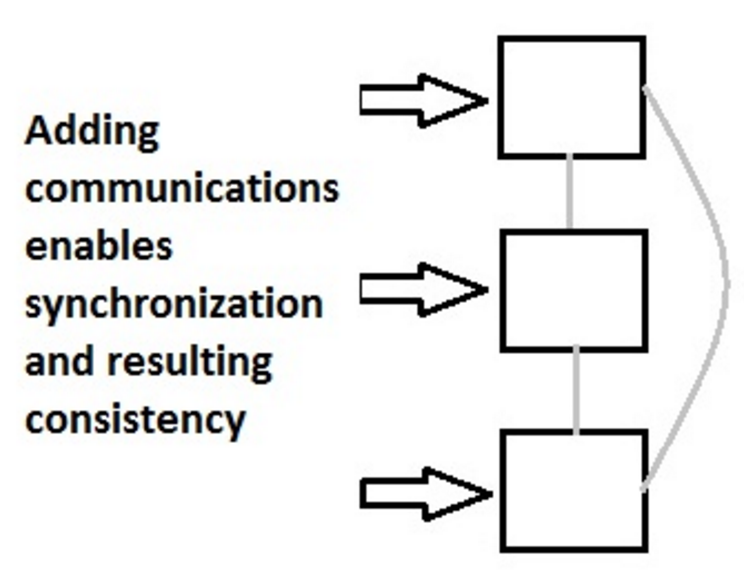
\includegraphics[width=0.5\textwidth]{img/ch07-consist.png}
\caption{Take consistency back.}
\label{fig:ch07-consist}
\end{figure}
But, notice what has happened. We gained consistency through communication. If we break that communication, we're back where we started. So, we now have consistency and availability, but not also partition tolerance. This is the "CA"/"AC" case.
\\

What about the "PC"/"CP" case? How can we have consistency and partition tolerance without availability, at least in any meaningful way? One ansewer, which is I think a good example, is that we enable reads, but not updates. Now we have sacraficed the avaialability of writes in order to ensure maintaining consistency in light of a partitioning.

